\documentclass{beamer}
\usepackage{ctex, hyperref}
\usepackage[T1]{fontenc}

% other packages
\usepackage{latexsym,amsmath,xcolor,multicol,booktabs,calligra}
\usepackage{graphicx,pstricks,listings,stackengine}

\nocite{*}

\author{杨占武}
\setbeamerfont{title}{size=\large}
\title{ns-3经验分享}
% \subtitle{毕业设计答辩}
\institute{大连理工大学软件学院}
\date{2024年5月20日}
\usepackage{dlut}

% defs
\def\cmd#1{\texttt{\color{red}\footnotesize $\backslash$#1}}
\def\env#1{\texttt{\color{blue}\footnotesize #1}}
\definecolor{deepblue}{rgb}{0,0,0.5}
\definecolor{deepred}{rgb}{0.6,0,0}
\definecolor{deepgreen}{rgb}{0,0.5,0}
\definecolor{halfgray}{gray}{0.55}

\lstset{
    basicstyle=\ttfamily\small,
    keywordstyle=\bfseries\color{deepblue},
    emphstyle=\ttfamily\color{deepred},    % Custom highlighting style
    stringstyle=\color{deepgreen},
    numbers=left,
    numberstyle=\small\color{halfgray},
    rulesepcolor=\color{red!20!green!20!blue!20},
    frame=shadowbox,
    morecomment=[l][\color{magenta}]{\#}, % 预处理器指令风格
    breaklines=true,            % 自动换行
    showspaces=false,           % 不显示空格
    showstringspaces=false      % 字符串中不显示空格
}


\begin{document}

\kaishu
\begin{frame}
	\titlepage
	\begin{figure}[htpb]
		\begin{center}
			\includegraphics[width=0.2\linewidth]{pic/DLUT-logo.eps}
		\end{center}
	\end{figure}
\end{frame}

\begin{frame}
	\tableofcontents[sectionstyle=show,subsectionstyle=show/shaded/hide,subsubsectionstyle=show/shaded/hide]
\end{frame}


\section{ns-3概述}

% \begin{frame}{}
% 	\begin{itemize}[<+-| alert@+>] % 当然,除了alert,手动在里面插 \pause 也行
% 		\item 大家都会\LaTeX{},好多学校都有自己的Beamer主题
% 		\item 中文支持请选择 Xe\LaTeX{} 编译选项
% 		\item GitHub项目地址位于 \url{https://github.com/fuujiro/dlut-Beamer-Slide},如果有bug或者feature request可以去里面提issue
% 	\end{itemize}
% \end{frame}

% \subsection{简介}

\begin{frame}{简介}
	\begin{columns}
		\column{.5\textwidth}
		\begin{itemize}
			\item 离散事件网络模拟器
			\item 模块化设计,便于扩展
			\item 免费的开源软件,文档详尽
			\item 代码晦涩难懂,学习曲线陡峭
			\item 开发环境推荐:Linux+Vscode+Copilot
		\end{itemize}

		\column{.5\textwidth}
		\begin{figure}[h]
			\centering
			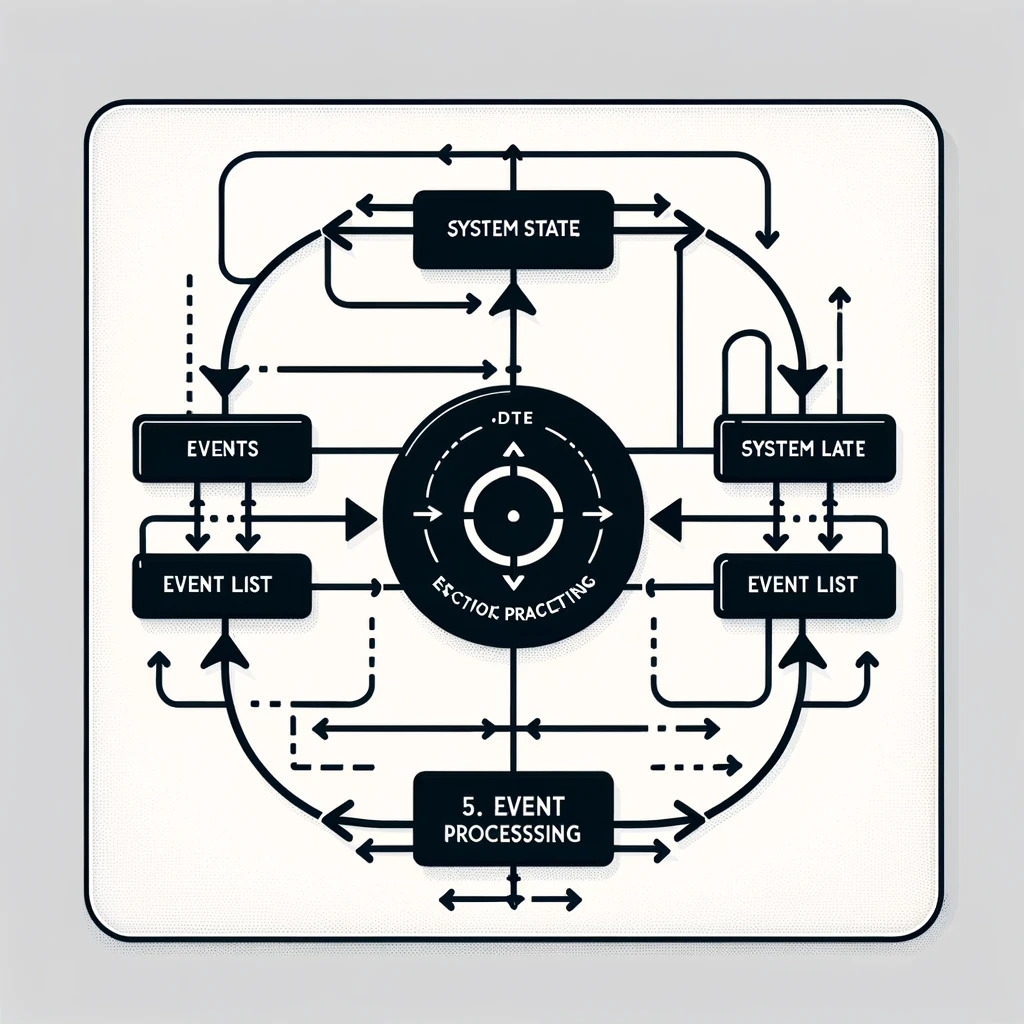
\includegraphics[height=0.5\textheight]{pic/events.png}
			\caption{事件示意图}
		\end{figure}

	\end{columns}
\end{frame}


\section{ns-3基础}

\subsection{关键抽象}

\begin{frame}
	\begin{columns}
		\column{.5\textwidth}
		\begin{itemize}
			\item Node,基本计算设备的抽象
			\item Application,生成要模拟活动的用户程序的抽象
			\item Channel,数据在网络中传输的介质的抽象
			\item NetDevice,软件驱动程序和模拟硬件的抽象
			\item Topology Helpers,将Nodes设置Channel进行连接
		\end{itemize}

		\column{.5\textwidth}
		\begin{figure}[h]
			\centering
			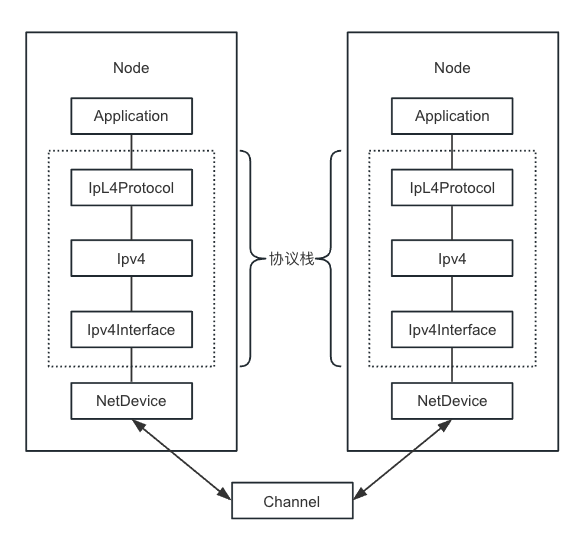
\includegraphics[height=0.7\textheight]{pic/ns3模型.png}
			\caption{ns-3模型}
		\end{figure}

	\end{columns}

\end{frame}

\subsection{仿真流程}

\begin{frame}
	\begin{itemize}
		\item 选择或开发相应的模块
		\item 编写网络仿真脚本
		      \begin{enumerate}
			      \item 生成节点,ns-3 中节点相当于一个空的计算机外壳
			      \item 安装网卡设备,不同的网络类型有不同的网络设备,从而提供不同的通信、物理层和 MAC 层
			      \item 安装协议栈,ns-3 网络中一般是 TCP/IP 协议栈
			      \item 安装应用层协议,依据选择的传输层协议选择相应的应用层协议
			      \item 其他配置:如节点是否移动,是否需要能量管理等
			      \item 启动仿真:整个网络场景配置完毕,启动仿真
			      \item debug:查看仿真结果,分析问题,这步相当痛苦
		      \end{enumerate}
	\end{itemize}
\end{frame}

\subsection{网络性能测试}

\begin{frame}{性能评判标准}
	\begin{itemize}
		\item 吞吐量:在单位时间内通过某个网络的实际的数据量
		\item 时延:数据从信源发送到信宿所需的时间
		\item 交付率:实际接收的数据包 / 总共发送的数据包
		\item 丢包率:1 - 交付率
		\item 能耗:一段时间内消耗的能量
		\item 路径长度:路由的跳数
	\end{itemize}
\end{frame}

\begin{frame}[fragile]{关键实现}
	回调函数
	\begin{lstlisting}[language=C++]
template <typename R, typename... Args>
Callback<R, Args...>
MakeCallback(R (*fnPtr)(Args...))
{
    return Callback<R, Args...>(fnPtr);
}

source->TraceConnectWithoutContext
("Tx", MakeCallback(&TxPacket));
sink->TraceConnectWithoutContext("Rx",MakeCallback
(&MacCompareExample::ReceivePacket, this));
\end{lstlisting}
\end{frame}

\begin{frame}[fragile]{关键实现}
	Schedule函数
	\begin{lstlisting}[language=C++]
template <typename... Us, typename... Ts>
EventId
Simulator::Schedule(const Time& delay, void (*f)(Us...), Ts&&... args)
{
    return DoSchedule(delay, MakeEvent(f, std::forward<Ts>(args)...));
}

Simulator::Schedule(Seconds(TotalTime / 100), &PrintProgress, TotalTime);
\end{lstlisting}
\end{frame}


\section{部分模块详解}

\subsection{Application代码讲解}
\begin{frame}[fragile]{OnOffApplication}
	\begin{lstlisting}[language=C++]
void
OnOffApplication::ScheduleNextTx()
{
    if (m_maxBytes == 0 || m_totBytes < m_maxBytes)
    {
        uint32_t bits = m_pktSize * 8 - m_residualBits;
        Time nextTime(Seconds(bits / static_cast<double>(m_cbrRate.GetBitRate())));
        m_sendEvent = Simulator::Schedule(nextTime, &OnOffApplication::SendPacket, this);
    }
}
\end{lstlisting}
\end{frame}

\begin{frame}[fragile]{PacketSink}
	\begin{lstlisting}[language=C++]
void HandleRead(Ptr<Socket> socket);

void HandleAccept(Ptr<Socket> socket, const Address& from);

void HandlePeerClose(Ptr<Socket> socket);

void HandlePeerError(Ptr<Socket> socket);

void PacketReceived(const Ptr<Packet>& p, const Address& from, const Address& localAddress);
\end{lstlisting}
\end{frame}

\subsection{Wifi模型}
\begin{frame}{模块实现}
	\begin{itemize}
		\item PHY层模型:模拟特定修正案和共有的PHY层操作和功能
		\item MAC低层模型:
		      \begin{enumerate}
			      \item FrameExchangeManager:处理帧交换序列,帧聚合、帧重传、保护和确认
			      \item ChannelAccessManager:实现了DCF和EDCAF功能
			      \item Txop 和 QosTxop:处理数据包队列
		      \end{enumerate}
		\item MAC高层模型:实现了Wifi中非时间关键的过程,如MAC层的信标生成、探测和关联状态机,以及一系列速率控制算法。
	\end{itemize}
\end{frame}

\subsection{网络层}
\begin{frame}[fragile]{模块实现}
	\begin{lstlisting}[language=C++]
int Socket::Send(const uint8_t* buf, uint32_t size, uint32_t flags);
int UdpSocketImpl::Send(Ptr<Packet> p, uint32_t flags);
int UdpSocketImpl::DoSendTo(Ptr<Packet> p, Ipv4Address dest, uint16_t port, uint8_t tos);
route = ipv4->GetRoutingProtocol()->RouteOutput(p, header, oif, errno_);
m_udp->Send(p->Copy(),header.GetSource(),header.GetDestination(),m_endPoint->GetLocalPort(),port,route);

void Ipv4Interface::Send(Ptr<Packet> p, const Ipv4Header& hdr, Ipv4Address dest);
\end{lstlisting}
\end{frame}

\subsection{MAC层与物理层}
\begin{frame}{模块实现}
	\begin{figure}[h]
		\centering
		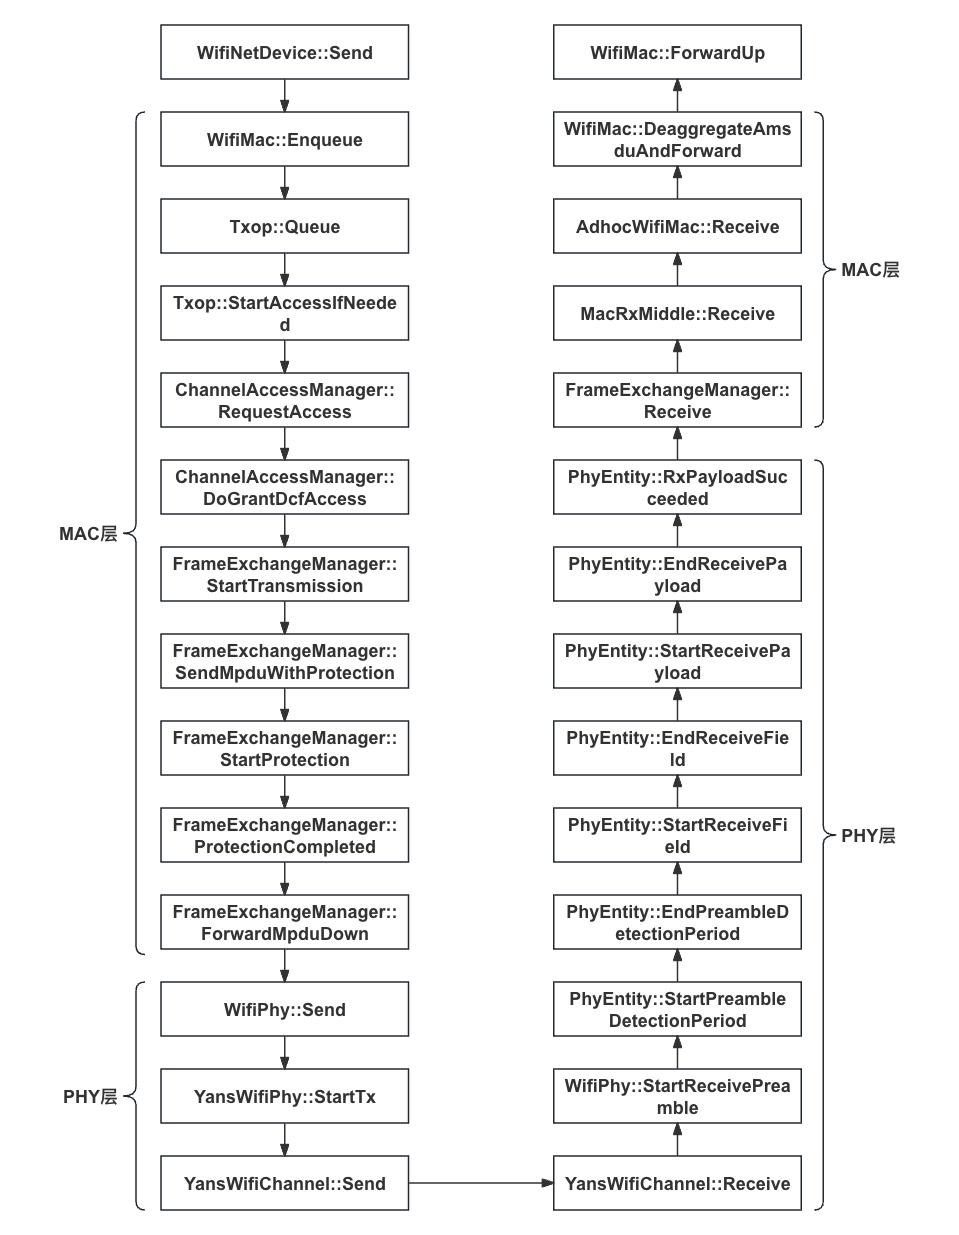
\includegraphics[height=0.8\textheight]{pic/数据流.png}
		\caption{数据传递流程图}
	\end{figure}
\end{frame}

\subsection{Channel模块}
\begin{frame}{模块实现}
	\begin{figure}[h]
		\centering
		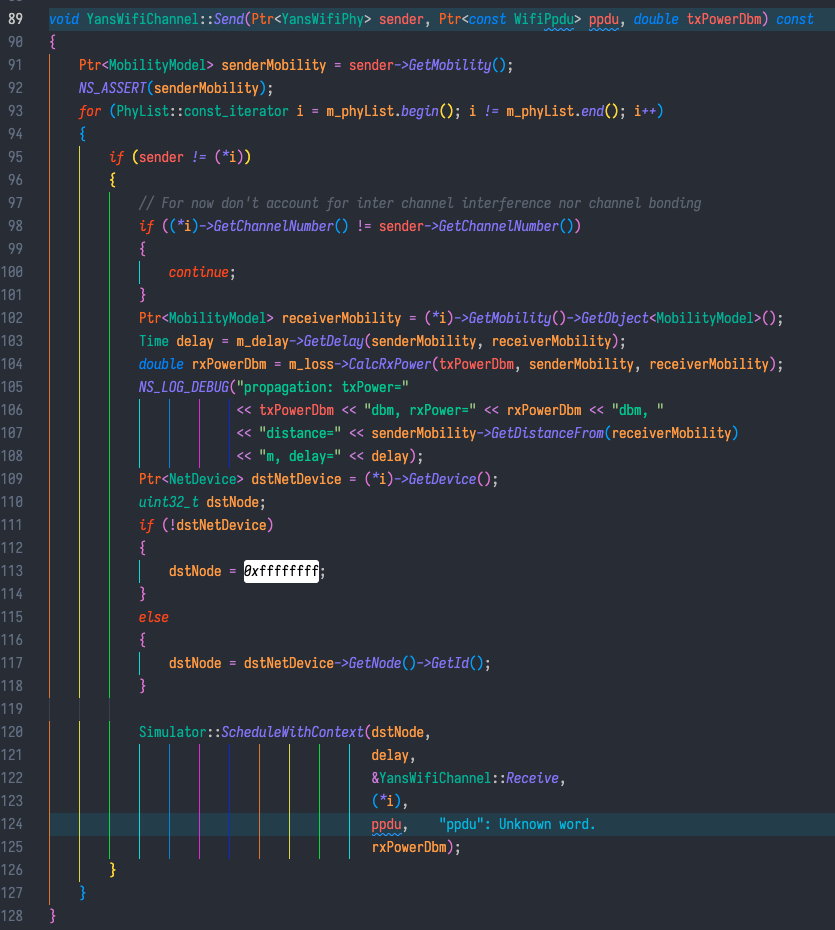
\includegraphics[height=0.8\textheight]{pic/channel.png}
		\caption{Channel模块关键函数}
	\end{figure}
\end{frame}

\subsection{损失模型修改}
\begin{frame}{模块实现}
	\begin{figure}[h]
		\centering
		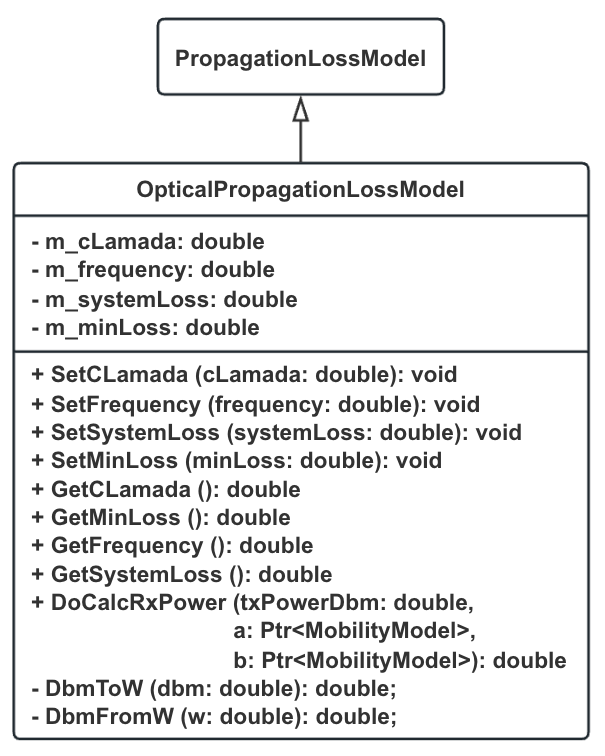
\includegraphics[height=0.8\textheight]{pic/传播衰减模型.png}
		\caption{传播衰减模型}
	\end{figure}
\end{frame}

\subsection{定向发送的实现}
\begin{frame}{模块实现}
	\begin{figure}[h]
		\centering
		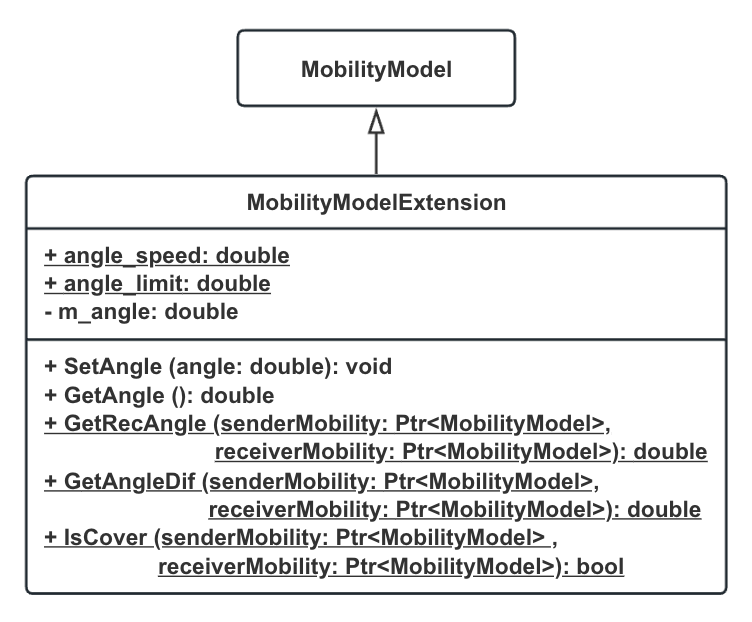
\includegraphics[height=0.8\textheight]{pic/MobilityModel.png}
		\caption{定向发送模型}
	\end{figure}
\end{frame}

% \begin{frame}{排版举例}
% 	\begin{exampleblock}{无编号公式} % 加 * 
% 		\begin{equation*}
% 			J(\theta) = \mathbb{E}_{\pi_\theta}[G_t] = \sum_{s\in\mathcal{S}} d^\pi (s)V^\pi(s)=\sum_{s\in\mathcal{S}} d^\pi(s)\sum_{a\in\mathcal{A}}\pi_\theta(a|s)Q^\pi(s,a)
% 		\end{equation*}
% 	\end{exampleblock}
% 	\begin{exampleblock}{多行多列公式\footnote{如果公式中有文字出现,请用 $\backslash$mathrm\{\} 或者 $\backslash$text\{\} 包含,不然就会变成 $clip$,在公式里看起来比 $\mathrm{clip}$ 丑非常多。}}
% 		% 使用 & 分隔
% 		\begin{align}
% 			Q_\mathrm{target} & =r+\gamma Q^\pi(s^\prime, \pi_\theta(s^\prime)+\epsilon)  \\
% 			\epsilon          & \sim\mathrm{clip}(\mathcal{N}(0, \sigma), -c, c)\nonumber
% 		\end{align}
% 	\end{exampleblock}
% \end{frame}

% \begin{frame}
% 	\begin{exampleblock}{编号多行公式}
% 		% Taken from Mathmode.tex
% 		\begin{multline}
% 			A=\lim_{n\rightarrow\infty}\Delta x\left(a^{2}+\left(a^{2}+2a\Delta x+\left(\Delta x\right)^{2}\right)\right.\label{eq:reset}\\
% 			+\left(a^{2}+2\cdot2a\Delta x+2^{2}\left(\Delta x\right)^{2}\right)\\
% 			+\left(a^{2}+2\cdot3a\Delta x+3^{2}\left(\Delta x\right)^{2}\right)\\
% 			+\ldots\\
% 			\left.+\left(a^{2}+2\cdot(n-1)a\Delta x+(n-1)^{2}\left(\Delta x\right)^{2}\right)\right)\\
% 			=\frac{1}{3}\left(b^{3}-a^{3}\right)
% 		\end{multline}
% 	\end{exampleblock}
% \end{frame}

% \begin{frame}{图形与分栏}
% 	% From thuthesis user guide.
% 	\begin{minipage}[c]{0.3\linewidth}
% 		\psset{unit=0.8cm}
% 		\begin{pspicture}(-1.75,-3)(3.25,4)
% 			\psline[linewidth=0.25pt](0,0)(0,4)
% 			\rput[tl]{0}(0.2,2){$\vec e_z$}
% 			\rput[tr]{0}(-0.9,1.4){$\vec e$}
% 			\rput[tl]{0}(2.8,-1.1){$\vec C_{ptm{ext}}$}
% 			\rput[br]{0}(-0.3,2.1){$\theta$}
% 			\rput{25}(0,0){%
% 				\psframe[fillstyle=solid,fillcolor=lightgray,linewidth=.8pt](-0.1,-3.2)(0.1,0)}
% 			\rput{25}(0,0){%
% 				\psellipse[fillstyle=solid,fillcolor=yellow,linewidth=3pt](0,0)(1.5,0.5)}
% 			\rput{25}(0,0){%
% 				\psframe[fillstyle=solid,fillcolor=lightgray,linewidth=.8pt](-0.1,0)(0.1,3.2)}
% 			\rput{25}(0,0){\psline[linecolor=red,linewidth=1.5pt]{->}(0,0)(0.,2)}
% 			%           \psRotation{0}(0,3.5){$\dot\phi$}
% 			%           \psRotation{25}(-1.2,2.6){$\dot\psi$}
% 			\psline[linecolor=red,linewidth=1.25pt]{->}(0,0)(0,2)
% 			\psline[linecolor=red,linewidth=1.25pt]{->}(0,0)(3,-1)
% 			\psline[linecolor=red,linewidth=1.25pt]{->}(0,0)(2.85,-0.95)
% 			\psarc{->}{2.1}{90}{112.5}
% 			\rput[bl](.1,.01){C}
% 		\end{pspicture}
% 	\end{minipage}\hspace{1cm}
% 	\begin{minipage}{0.5\linewidth}
% 		\medskip
% 		%\hspace{2cm}
% 		\begin{figure}[h]
% 			\centering
% 			\includegraphics[height=.4\textheight]{pic/dtmf.pdf}
% 		\end{figure}
% 	\end{minipage}
% \end{frame}

% \begin{frame}[fragile]{\LaTeX{} 常用命令}
% 	\begin{exampleblock}{命令}
% 		\centering
% 		\footnotesize
% 		\begin{tabular}{llll}
% 			\cmd{chapter}   & \cmd{section} & \cmd{subsection} & \cmd{paragraph}       \\
% 			章               & 节             & 小节               & 带题头段落                 \\\hline
% 			\cmd{centering} & \cmd{emph}    & \cmd{verb}       & \cmd{url}             \\
% 			居中对齐            & 强调            & 原样输出             & 超链接                   \\\hline
% 			\cmd{footnote}  & \cmd{item}    & \cmd{caption}    & \cmd{includegraphics} \\
% 			脚注              & 列表条目          & 标题               & 插入图片                  \\\hline
% 			\cmd{label}     & \cmd{cite}    & \cmd{ref}                                \\
% 			标号              & 引用参考文献        & 引用图表公式等                                  \\\hline
% 		\end{tabular}
% 	\end{exampleblock}
% 	\begin{exampleblock}{环境}
% 		\centering
% 		\footnotesize
% 		\begin{tabular}{lll}
% 			\env{table}   & \env{figure}    & \env{equation}    \\
% 			表格            & 图片              & 公式                \\\hline
% 			\env{itemize} & \env{enumerate} & \env{description} \\
% 			无编号列表         & 编号列表            & 描述                \\\hline
% 		\end{tabular}
% 	\end{exampleblock}
% \end{frame}

% \begin{frame}[fragile]{\LaTeX{} 环境命令举例}
% 	\begin{minipage}{0.5\linewidth}
% 		\begin{lstlisting}[language=TeX]
% \begin{itemize}
%   \item A \item B
%   \item C
%   \begin{itemize}
%     \item C-1
%   \end{itemize}
% \end{itemize}
% \end{lstlisting}
% 	\end{minipage}\hspace{1cm}
% 	\begin{minipage}{0.3\linewidth}
% 		\begin{itemize}
% 			\item A
% 			\item B
% 			\item C
% 			      \begin{itemize}
% 				      \item C-1
% 			      \end{itemize}
% 		\end{itemize}
% 	\end{minipage}
% 	\medskip
% 	\pause
% 	\begin{minipage}{0.5\linewidth}
% 		\begin{lstlisting}[language=TeX]
% \begin{enumerate}
%   \item 巨佬 \item 大佬
%   \item 萌新
%   \begin{itemize}
%     \item[n+e] 瑟瑟发抖
%   \end{itemize}
% \end{enumerate}
% \end{lstlisting}
% 	\end{minipage}\hspace{1cm}
% 	\begin{minipage}{0.3\linewidth}
% 		\begin{enumerate}
% 			\item 巨佬
% 			\item 大佬
% 			\item 萌新
% 			      \begin{itemize}
% 				      \item[n+e] 瑟瑟发抖
% 			      \end{itemize}
% 		\end{enumerate}
% 	\end{minipage}
% \end{frame}

% \begin{frame}[fragile]{\LaTeX{} 数学公式}
% 	\begin{columns}
% 		\begin{column}{.55\textwidth}
% 			\begin{lstlisting}[language=TeX]
% $V = \frac{4}{3}\pi r^3$

% \[
%   V = \frac{4}{3}\pi r^3
% \]

% \begin{equation}
%   \label{eq:vsphere}
%   V = \frac{4}{3}\pi r^3
% \end{equation}
% \end{lstlisting}
% 		\end{column}
% 		\begin{column}{.4\textwidth}
% 			$V = \frac{4}{3}\pi r^3$
% 			\[
% 				V = \frac{4}{3}\pi r^3
% 			\]
% 			\begin{equation}
% 				\label{eq:vsphere}
% 				V = \frac{4}{3}\pi r^3
% 			\end{equation}
% 		\end{column}
% 	\end{columns}
% 	\begin{itemize}
% 		\item 更多内容请看 \href{https://zh.wikipedia.org/wiki/Help:数学公式}{\color{purple}{这里}}
% 	\end{itemize}
% \end{frame}

% \begin{frame}[fragile]
% 	\begin{columns}
% 		\column{.6\textwidth}
% 		\begin{lstlisting}[language=TeX]
%     \begin{table}[htbp]
%       \caption{编号与含义}
%       \label{tab:number}
%       \centering
%       \begin{tabular}{cl}
%         \toprule
%         编号 & 含义 \\
%         \midrule
%         1 & 4.0 \\
%         2 & 3.7 \\
%         \bottomrule
%       \end{tabular}
%     \end{table}
%     公式~(\ref{eq:vsphere}) 的
%     编号与含义请参见
%     表~\ref{tab:number}。
% \end{lstlisting}
% 		\column{.4\textwidth}
% 		\begin{table}[htpb]
% 			\centering
% 			\caption{编号与含义}
% 			\label{tab:number}
% 			\begin{tabular}{cl}\toprule
% 				编号 & 含义  \\\midrule
% 				1  & 4.0 \\
% 				2  & 3.7 \\\bottomrule
% 			\end{tabular}
% 		\end{table}
% 		\normalsize 公式~(\ref{eq:vsphere})的编号与含义请参见表~\ref{tab:number}。
% 	\end{columns}
% \end{frame}

% \begin{frame}{作图}
% 	\begin{itemize}
% 		\item 矢量图 eps, ps, pdf
% 		      \begin{itemize}
% 			      \item METAPOST, pstricks, pgf $\ldots$
% 			      \item Xfig, Dia, Visio, Inkscape $\ldots$
% 			      \item Matlab / Excel 等保存为 pdf
% 		      \end{itemize}
% 		\item 标量图 png, jpg, tiff $\ldots$
% 		      \begin{itemize}
% 			      \item 提高清晰度,避免发虚
% 			      \item 应尽量避免使用
% 		      \end{itemize}
% 	\end{itemize}
% 	\begin{figure}[htpb]
% 		\centering
% 		\includegraphics[width=0.2\linewidth]{pic/DLUT-logo.eps}
% 		\caption{这个校徽就是矢量图}
% 	\end{figure}
% \end{frame}


% \section{模块修改}
% \begin{frame}
% 	\begin{itemize}
% 		\item 一月:完成文献调研
% 		\item 二月:复现并评测各种Beamer主题美观程度
% 		\item 三、四月:美化dlut Beamer主题
% 		\item 五月:论文撰写
% 	\end{itemize}
% \end{frame}


\section{资料推荐}

\begin{frame}{个人推荐}
	\bibliography{ref}
	\bibliographystyle{alpha}
	\textbf{推荐至少预留2周时间实验}

	ns-3官方文档
	\begin{itemize}
		\item \href{https://www.nsnam.org/documentation/}{https://www.nsnam.org/documentation/}
	\end{itemize}
	ns-3技术博客
	\begin{itemize}
		\item \href{https://jluyeyu.com/categories/ns3/}{https://jluyeyu.com/categories/ns3/}
		\item \href{https://www.jianshu.com/p/8d419dae1f9f}{https://www.jianshu.com/p/8d419dae1f9f/}
	\end{itemize}
	gdb入门
	\begin{itemize}
		\item \href{https://gitsang.github.io/docs/cpp/gdb\_quick\_start}{https://gitsang.github.io/docs/cpp/gdb\_quick\_start/}
	\end{itemize}

\end{frame}

\begin{frame}
	\begin{center}
		{\Huge\calligra Thanks!}
	\end{center}
\end{frame}

\end{document}